% !TeX spellcheck = en_US
% !TeX root = notes.tex
\subsection{Adaptability and self-management in DS}
\subsubsection{Using interceptors to adapt control}
\begin{itemize}
	\item Interceptors change flow of control and allow additional code to be executed
	\item Many object-based DS use interceptors to change flow of control in the object invocation
	\subitem Requests (object invocations) can be intercepted
	\subitem Messages can be intercepted	
\end{itemize}
\subsubsection{General Approaches to Adaptive Software}
\begin{itemize}
	\item\textbf{Separation of concerns}
	\subitem e.g. \textit{aspect oriented programming} (not very successful)
	\item\textbf{Computational reflection}
	\subitem e.g. \textit{reflective middleware}
	\item\textbf{Component-based design}
	\subitem Adaptation through composition
	\subsubitem Statically at design time
	\subsubitem Dynamically at run time (requires support for late binding)	
\end{itemize}

\subsubsection{The Feedback Control Model}
\begin{figure}[H]
	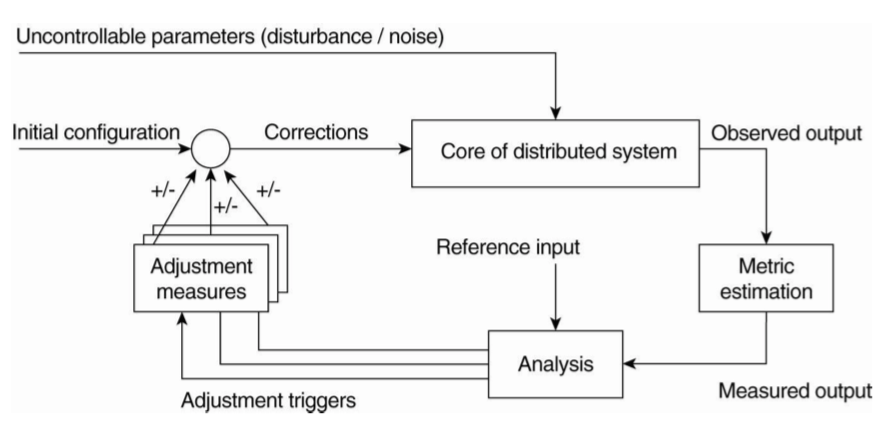
\includegraphics[width=0.8\linewidth]{feedback}	
	\centering\caption{The logical organisation of a feedback control system}
\end{figure}



\subsection{Processes}
\begin{note}{Core OS functionality}
	\begin{itemize}
		\item Process Manager
		\subitem Process lifecycle
		\item Thread Manager
		\subitem Thread lifecycle
		\item Communication Manager
		\subitem Communication between threads attached to different process
		\item Memory Manager
		\subitem Physical/virtual
		\item Supervisor
		\subitem Dispatching interrupts, traps, ...	
	\end{itemize}
\end{note}

\subsubsection{Definitions}
\begin{itemize}
	\item\textbf{Process}
	\begin{itemize}
		\item Program being executed
		\item Consists of address space and execution state (program counter, stack pointer, processor status word, contents of registers and system-call state)
	\end{itemize}
	\item\textbf{Thread} (of execution)
	\begin{itemize}
		\item Abstraction of activity within process
	\end{itemize}
\end{itemize}
Thread has less overhead and so interruptions and switching can be faster. Threads also have shared memory

\subsubsection{Multithreaded Servers}
\begin{description}
	\item[Threads:] Parallelism, blocking system calls
	\item[Single-threaded process:] No parallelism, blocking system calls
	\item[Finite-state machine:] Parallelism, nonblocking system calls
\end{description}


\subsubsection{Virtualisation in DS}
\textit{Interface at different levels:}
\begin{enumerate}
	\item An interface between the hardware and software consisting of machine instructions
	\subitem that can be invoked by any program
	\item An interface between the hardware and software, consisting of machine instructions
	\subitem that can be invoked only by privileged programs, such as an operating system
	\item An interface consisting of system calls as offered by an operating system
	\item An interface consisting of library calls
	\subitem generally forming what is known as an application programming interface (API)
	\subitem in many cases, system calls are hidden by an API
\end{enumerate}

\subsubsection{Clients/Servers}
\begin{itemize}
	\item Clients are often \textbf{thin}
	\subitem Large portion of processing required to support sophisticated user interfaces can by provided by servers	
	\item Clients should support transparencies
	\subitem communication hiding
	\subitem access transparency (client stub)
	\subitem location, migration, relocation transparencies
\end{itemize}

\paragraph{Servers General Design Issues}
\begin{description}
	\item[Stateful server:] maintains information on clients
	\subitem hard to handle failures
	\item[Stateless server:] knows nothing about clients
	\subitem can change own state without informing clients
\end{description}
